\chapter{数列和数列求和}

\section{数列的概念}
\subsection{数列的定义}

首先让我们再来看一看人类最先认识的数——自然数:$1,2,3,4,\ldots,n,n+1,\ldots$, 它们是一串依次排列的数,从 1 开始\footnote{在这套教材编写之时,0 还不被包括在自然数集之内,因此,本教材里所述的自然数实际为正整数。},逐次加 1 至无穷,这就是本节要讲的数列的一个原始的例子。下面再举几个数列的例子:

\begin{example}\label{exp:natural_number}
    在自然数里,把被 3 整除,被 3 除余 1,被 3 除余 2 的那些数,分别由小到大排列成数列。
\end{example}

\begin{solution}
    被 3 整除的数:$3,\,3\times2,\,3\times3,\,3\times4,\,\ldots,\,3n,\,3(n+1),\ldots$

被 3 除余1的数:$3+1,\,3\times2+1,\,3\times3+1,\,3\times4+1,\,\ldots,\,3n+1,\,3(n+1)+1,\,\ldots$

被 3 除余 2 的数:$3+2,\,3\times2+2,\,3\times3+2,\,3\times4+2,\,\ldots , 3n+2,\,3(n+1) +2,\,\ldots$
\end{solution}

\begin{example}\label{exp:rabbit}
  某人考察,一对兔子经过一年的繁殖,总共可以有多少对兔子,假设兔子的生殖力是这样的:每一对兔子每一个月可以生一对兔子,并且兔子在生出两个月以后就具有生殖后代的能力,在各月份里观察到的兔子的对数如下表所示:
\begin{table}
\begin{tblr}{colspec={c*{12}{X[r]}},hline{2}=0.8pt}
$n$&1&2&3&4&5&6&7&8&9&10&11&12\\
$u_n$&2&3&5&8&13&21&34&55&89&144&233&377\\
\end{tblr}
\end{table}

设 $n$ 代表月份,$u_n$ 代表该月内兔子对数。在第一个月里,第一对兔子生了一对后代,因此 $u_1=2$, 在这两对中,只有第一对能够在下一个月里生一对兔子,所以 $u_2=3$,以后各月的兔子总对数除了上一个月的兔子总对数外,再加上其中又能够在这个月产生后代的兔子对数,即前一个月的兔子的总对数,因此以后各月的兔子总对数可以由公式:
\[u_n=u_{n-1}+u_{n-2},\qquad (2< n\leqslant 12)\]
计算出来。
\end{example}

\begin{example}\label{exp:fraction}
试将 $\dfrac{1}{7}$ 准确到 $\dfrac{1}{10},\,\dfrac{1}{10^2},\,\dfrac{1}{10^3},\ldots$ 的不足近似值和过剩近似值分别排成数列。
\end{example}

\begin{solution}
  {\linespread{1.60}\selectfont
  将 $\dfrac{1}{7}$ 化成无限循环小数得到 $1/7=0.\dot{1}4285\dot{7}$. 如果分别按去尾法和进一法舍取近似数,就是说,取 $0.\dot{1}4285\dot{7}$ 前 $n$ 个数位上的数码而把它后面尾部数码都舍去,这样得到的有限小数 $u_n^-$ 叫做 $\dfrac{1}{7}$ 的准确到 $\dfrac{1}{10^n}$ 的不足近似值,而把 $u_n^+=u_n^-+\dfrac{1}{10^n}$ 叫做 $1/7$ 的准确到 $\dfrac{1}{10^n}$ 的过剩近似值。\par\medskip}

由 $\dfrac{1}{7}$ 的准确到 $\dfrac{1}{10^n}$ 的不足近似值组成的数列是
\[0.1,\; 0.14,\; 0.142,\; 0.1428,\; 0.14285,\ldots\]
由 $\dfrac{1}{7}$ 的准确到 $\dfrac{1}{10^n}$ 的过剩近似值组成的数列是
\[0.2,\; 0.15,\; 0.143,\; 0.1429,\; 0.14286,\ldots\]
显然有:
\[\begin{split}
   & 0.1<0.14<0.142<0.1428<0.14285<\cdots<\frac{1}{7}\\
   &\qquad <\cdots<
0.14286<0.1429<0.143<0.15<0.2
\end{split}\]
并且
\[\left|u_n^--\frac{1}{7} \right|<\frac{1}{10^n},\qquad \left|u_n^+-\frac{1}{7} \right|<\frac{1}{10^n}\]
\end{solution}

现在我们可以给数列下个定义如下:
\begin{Definition}
一串依次排列的数 $a_1,a_2,\ldots,a_n,\ldots$ 叫做\emph{数列}。

数列中的数,叫做数列的\emph{项},用 $a_n$ 表示,每一项的位置序数 $n$ 叫做该项的\emph{指标},通常写在 $a$ 的右下角,故也叫\emph{下标}。数列用符号 $\{a_n,\; n=1,2,3,\ldots\}$ 表示,或简写为 $\{a_n\}$。
\end{Definition}

依定义,数列就是对每一个自然数 $n$ 指定一项 $a_n$,换言之,数列就是自然数的函数。

通过前面的例子知道,我们可以用以下几种方式给出一个数列:
\begin{enumerate}
\item 给出一个以指标$n$表示数列的任意一项 $a_n$ 的公式,这公式叫做数列的\emph{通项公式}。例如在\cref{exp:natural_number} 中,数列的通项公式分别是
\[a_n=3n,\quad b_n=3n+1,\quad c_n=3n+2 \quad (n=1,2,3,\ldots)\]
\item 有的数列从某一项开始能够用在它前面的 $k$ 个项表示出来。这个表达式叫做\emph{递归方程}。例如\cref{exp:rabbit} 中的数列,由两个初始值 $u_1=2$, $u_2=3$ 和一个递归方程给出:
\[u_n=u_{n-1}+u_{n-2},\qquad (n=3,4,5,\ldots,12)\]
\item 有的数列直接用语言描述它的 $a_n$ 项,用来作一般性的讨论,如\cref{exp:fraction} 中的数列。
\end{enumerate}

\subsection{数列的种类及其定义}
\subsubsection{有穷数列和无穷数列}
有末项的数列叫做\emph{有穷数列},无末项的数列叫做\emph{无穷数列}。如\cref{exp:rabbit} 的数列是有穷数列,\cref{exp:natural_number,exp:fraction} 的数列是无穷数列。

\subsubsection{单调数列和摆动数列}

数列 $\{a_n\}$ 中的项,若满足不等式
\begin{itemize}
  \item $a_{n+1}\geqslant a_n,\quad (n=1,2,3,4,\ldots,n,\ldots)$, 那么数列叫做\emph{不减的}; 
  \item 如果 $a_{n+1}> a_n,\quad (n=1,2,3,4,\ldots,n,\ldots)$,那么数列叫做\emph{递增的};
  \item 如果 $a_{n+1}= a_n,\quad (n=1,2,3,4,\ldots,n,\ldots)$,那么数列叫做\emph{常数列};
  \item 如果 $a_{n+1}\leqslant a_n,\quad (n=1,2,3,4,\ldots,n,\ldots)$,那么数列叫做\emph{不增的};
  \item 如果 $a_{n+1}< a_n,\quad (n=1,2,3,4,\ldots,n,\ldots)$,那么数列叫\emph{递减的}。
\end{itemize}

以上各种数列统称为\emph{单调数列}。

数列 $\{a_n\}$ 中的项,如果总有一些项大于前面的项,又总有一些项小于前面的项,那么数列叫做\emph{摆动数列}。

例如:以下数列都是摆动数列
\begin{itemize}
  \item 数列 $\{(-1)^{n+1}\}$:$1,-1,1,-1,\ldots$
  \item 数列 $a_n=\begin{cases}
    \dfrac{1}{n}, & \text{$n$是奇数}\\
    \dfrac{n}{n+1}, & \text{$n$是偶数}\\
  \end{cases}$:$1,\dfrac{2}{3},\dfrac{1}{3},\dfrac{4}{5},\dfrac{1}{5},\dfrac{6}{7},\ldots$
  \item 数列 $\{(-1)^{n}n\}$:$-1,2,-3,4,\ldots$
\end{itemize}

\subsubsection{有界数列和无界数列}
有穷数列一定有最大项和最小项,无穷数列就不一定有此性质。无穷数列可分成有界数列和无界数列。

\begin{Definition}
任何一项的绝对值都小于某一正数,即 $|a_n|<M,\quad (M>0)$ 的数列叫做\emph{有界数列};没有这样正数存在的数列
叫做\emph{无界数列}。    
\end{Definition}
 
例如,数列 $\{(-1)^n\}$和$\{n+(-1)^n n\}$ 都是无界数列。

数列 $\left\{(-1)^{n+1}\left(1+\dfrac{1}{n}\right)\right\}$ 是有界数列,因为
\[|a_n|=\left|(-1)^{n+1}\left(1+\frac{1}{n}\right)\right|=1+\frac{1}{n}\leqslant 2,\quad (n=1,
2,3,4,\ldots)\]

若数列递增,并且所有 $a_n\leqslant M$(定数),则称\emph{数列有上界} $M$。

\begin{Deduction}{推论 1}
  递增有上界数列一定是有界数列。
\end{Deduction}

若数列递减,并且所有 $a_n\geqslant M$(定数),则称\emph{数列有下界} $M$。

\begin{Deduction}{推论 2}
  递减有下界数列一定是有界数列。
\end{Deduction}

\begin{Deduction}{推论 3}
  有穷数列一定是有界数列。
\end{Deduction}

图示数列的最简单的方法是直接把点 $a_1,a_2,a_3,\ldots$ 标在数轴上,这种图象可以清楚地表示数列变化的状态和趋势。\cref{fig:series_graph} 是几个数列的图象。

\begin{figure}
\begin{tikzpicture}[>=stealth]
\begin{scope}
    \draw[->] (-0.5,0)--(8,0)node[above]{$\left\{\dfrac{n}{n+1}\right\}$};
    \foreach \x/\xtext in {{1/2}/a_1, {2/3}/a_2,   {3/4}/a_3,  {4/5}/a_4}
    {
        \draw (\x*7,0)--(\x*7,.1)node[above]{$\xtext$};
    }
\foreach \x in {0,1}
{
    \draw (\x*7,0)node[below]{$\x$}--(\x*7,.1);
}
\end{scope}    
\begin{scope}[yshift=-1.5cm]
    \draw[->] (-0.5,0)--(8,0)node[above]{$\left\{\left(\dfrac{1}{2}\right)^n\right\}$};   
    \foreach \x/\xtext in {{1/2}/a_1, {1/4}/a_2,   {1/8}/a_3,  {1/16}/a_4, {1/32}/a_5}
    {
        \draw (\x*14,0)--(\x*14,.1)node[above]{$\xtext$};
    }
\foreach \x/\xtext in {0/0,1/\frac{1}{2}}
{
    \draw (\x*7,0)node[below]{$\xtext$}--(\x*7,.1);
}
\end{scope}   
\begin{scope}[yshift=-3cm]
    \draw[->] (-0.5,0)--(8,0)node[above]{$\left\{\sin n\uppi\right\}$};
    \draw (0,0)node[below]{0}--(0,.1);
    \node at (-.2,.5)[right]{$a_1=a_2=a_3=\cdots$};
\end{scope}   
\begin{scope}[yshift=-4.5cm]
    \draw[->] (-0.5,0)--(8,0)node[above]{$\left\{(-1)^n n\right\}$};
    \foreach \x/\xtext  in {-5/a_5,-3/a_3,-1/a_1,2/a_2,4/a_4}
{
    \draw (\x*.7+3.5,0)--(\x*.7+3.5,.1)node[above]{$\xtext$};
}
\foreach \x in {-1,0}
{
    \draw (\x*.7+3.5,0)node[below]{$\x$}--(\x*.7+3.5,.1);
}


\end{scope}   
\begin{scope}[yshift=-6cm]
    \draw[->] (-0.5,0)--(8,0)node[above]{$\left\{n+(-1)^n n\right\}$};
    \node at (-.2,.5)[right]{$a_1=a_3=a_5=\cdots$};
    \foreach \x/\xtext  in {0/0, 2/a_2,4/a_4,6/a_6}
{
    \draw (\x*.5,0)node[below]{$\xtext$}--(\x*.5,.1);
}
\end{scope}   
\end{tikzpicture}
    \caption{}\label{fig:series_graph}
\end{figure}
 

\begin{Exercise}
\begin{question}
  \item 自然数里的质数由小到大排成一个数列,试依次写出它的前 10 个质数。
  \item 分别用通项公式表示由小到大排列着的偶数数列和奇数数列。
  \item 试写出下列各数列的通项公式
  \begin{tasks}(2)
    \task $1^2,\; 2^2,\; 3^2,\; 4^2,\; \ldots$
    \task $1,\; -\dfrac{1}{2},\; \dfrac{1}{2}-\dfrac{1}{3},\; \dfrac{1}{3}-\dfrac{1}{4},\; \ldots$
    \task $\dfrac{3}{2},\; \dfrac{4}{3},\; \dfrac{5}{4},\; \dfrac{6}{5},\; \ldots$
    \task $\dfrac{10}{3},\; \dfrac{20}{9},\; \dfrac{30}{27},\; \dfrac{40}{81},\; \ldots$
    \task $\dfrac{1\cdot 3}{2\cdot 4},\; \dfrac{3\cdot 5}{4\cdot 6},\; \dfrac{5\cdot 7}{6\cdot 8},\; \dfrac{7\cdot 9}{8\cdot 10},\; \ldots$
    \task $1,\; -\dfrac{1}{2},\; \dfrac{1}{3},\; -\dfrac{1}{4},\; \dfrac{1}{5},\; \ldots$
    \task $1,\; 1\cdot 2,\; 1\cdot 2\cdot 3,\; 1\cdot 2\cdot 3\cdot 4,\;\ldots $
    \task $\dfrac{1}{1\cdot 2},\; -\dfrac{1}{3\cdot 4},\; \dfrac{1}{5\cdot 6},\; -\dfrac{1}{7\cdot 8},\; \ldots$
  \end{tasks}
  \item 根据下列各数列的通项公式,写出它的前 10 项。
 \begin{tasks}%(2)
    \task $a_n=\cos n\uppi,\quad (n=1,2,3,\ldots)$
    \task $a_n=\dfrac{2+(-1)^n}{n},\quad (n=1,2,3,\ldots)$
    \task $f(n)=\begin{cases}
        \dfrac{1}{n},& \text{$n$ 为奇数}\\
        \dfrac{n}{n+1},& \text{$n$ 为偶数}\\
    \end{cases}$
\end{tasks}       

\item 试将所有整数排成一个数列,并且用通项公式表示出来。
\item 数列的通项公式是
\[f(n)=\frac{5+3\sqrt{5}}{10}\left(\frac{1+\sqrt{5}}{2}\right)^n+\frac{5-3\sqrt{5}}{10}\left(\frac{1-\sqrt{5}}{2}\right)^n,\quad (n=1,2,3,\ldots)\]
\begin{tasks}
  \task 求 $f(1)$, $f(2)$;
  \task 求证 $f(n)=f(n-1)+f(n-2)$.
\end{tasks}

\item 判断下列各数列的类型并图示它前 5 项。
\begin{tasks}
  \task $a_n=1-2n,\quad (n=1,2,3,\ldots,10)$;
  \task $a_n=\dfrac{2n+1}{n},\quad (n=1,2,3,\ldots)$;
  \task $a_n=\dfrac{(-1)^n2^n}{4},\quad (n=1,2,\ldots,5)$;
  \task! $a_n=\dfrac{(-1)^{n+1}n}{n+1},\quad (n=1,2,3,\ldots)$;
  \task* $\sqrt{2}$ 的准确到 $1,\; 0.1,\; 0.01,\; \ldots$ 的过剩近似值。
  \task* $a_n=\dfrac{2+(-1)^n}{n},\quad (n=1,2,3,\ldots)$;
  \task* $a_n=(-1)^n\left(\dfrac{n-1}{n+1}\right)^2,\quad (n=1,2,3,\ldots)$;
  \task $a_n=\dfrac{2n^2-3}{n},\quad (n=1,2,3,\ldots)$;
  \task $a_n=\dfrac{-2n^2-3}{n},\quad (n=1,2,3,\ldots)$;
  \task $a_n=\tan \dfrac{n\uppi}{3},\quad  (n=1,2,3,\ldots)$。
\end{tasks}
\item 数列的通项公式是
\[a_n=2n^2-3,\quad (n=1,2,3,\ldots)\]
求数列的第 5 项,下面三个数:84788、32352 和 72197中,哪个数是数列中的项,是第几项?
\end{question}
\end{Exercise}

\section{数列求和举例}
在本节,我们要复习第一册已经学习过的两个简单而重要的数列,即等差数列和等比数列,同时通过例题来说明几种常用的求数列前 $n$ 项和的方法。

如果一个数列,从第二项起,每一项减去它的前面的一项所得的差都等于同一个常数,那么这个数列叫做\emph{等差数列},这个常数叫做等差数列的\emph{公差},用符号 $d$ 表示。等差数列的通项公式是
\[a_n=a_1+(n-1)d,\qquad (n=1,2,3,\ldots)\]
它的前 $n$ 项求和公式是
\[S_n=\frac{n(a_1+a_n)}{2}\]
或
\[S_n=na_1+\frac{n(n-1)}{2}d\]
我们已在第一册给出上面求和公式的推导过程,现在建议读者独立地把它们推导出来,在通项公式与求和公式中共包含了五个数量:$a_1$, $d$, $n$, $a_n$ 和 $S_n$。如果问题给出了其中三个数量,那么其余两个数量便可由它们解出来。

\begin{example}
  在数轴上有两个点 $A(4.5)$ 和 $B(12.5)$,在其间插入四个等间隔的点,求这些点的坐标。
\end{example}

\begin{solution}
  在 $A$ 和 $B$ 两点之间插入四个等间隔的点后,这六个点的对应坐标成等差数列,

$\because\quad     a_1=4.5,\quad a_6=12.5,\quad n=6$

$\therefore\quad     12.5=4.5+(6-1)d$,解得:$d=1.6$。

所求四个点的坐标分别是 $6.1,\; 7.7,\; 9.3,\; 10.9$。
\end{solution}

\begin{Definition}
  给出两个数,其间插入一个数,使成等差数列,被插入的数叫做这二数的\emph{等差中项}。
\end{Definition}

\begin{Deduction}{推论}
  若 $a,b,c$ 三个数成等差数列,则等差中项 \[b=\frac{a+c}{2}\]
\end{Deduction}
 
事实上,依定义有
\[b-a=c-b\]
移项,得
\[2b=a+c\]
即
\[b=\frac{a+c}{2}\]
    
\begin{example}
  在甲地有 48 根电杆,从离甲地 1000 米的地方树立第一根电杆,以后每隔 15 米树立一根电杆,载重汽车每次只能拖运三根电杆,问由一辆汽车去完成任务至少需要行驶多少公里?
\end{example}

\begin{solution}
  汽车需运电杆 $48\div 3=16$ 次才能完成任务,所以,$n=16$。设 $a_n$ 为第 $n$ 次拖运电杆再返回原地所行驶的路程,依题意 $\{a_n\}$ 是等差数列,且知 
\[    a1=2060,\qquad d=90,\qquad n=16\]
因此:
\[\begin{split}
    S_n&=na_1+\frac{n(n-1)}{2}d\\
    &=16\times 2060+\frac{16\times 15}{2}\times 90\\
    &=43760\,\unit{(\text{米})}=43.76\,\unit{(\text{公里})}
\end{split}\]

答:汽车需行驶 43.76 公里,才能完成任务。
\end{solution}

\bigskip
如果一个数列,从第二项起,每一项和前面一项的比都等于一个常数,那么,这个数列叫做\emph{等比数列}。这个常数叫做等比数列的\emph{公比},通常用字母 $q$ 表示。换言之,等比数列是满足递归关系 $a_{n+1}=qa_{n},\quad (n=1,2,\ldots)$ 的数列。

显然,当 $q>0$ 时,等比数列是单调的。若 $q>1$,等比数列是递增的;若 $0<q<1$,等比数列是递减的;若 $q=1$,等比数列是常数列。

当 $q<0$ 时,等比数列是摆动的。

又当 $|q|\leqslant 1$ 时,等比数列是有界的,当 $|q|>1$ 时,等比数列是无界的。

我们已经知道等比数列的通项公式是
\[a_n=a_1q^{n-1}\qquad (n=1,2,\ldots)\]
它前 $n$ 项和公式是
\[S_n=\frac{a_nq-a_1}{q-1}\]
若 $q<1$,上式改写为
\[S_n=\frac{a_1-a_nq}{1-q}\]
显然,若 $q=1$,则 $S_n=na_1$。

将 $a_n=a_1q^{n-1}$ 代入求和公式中,得到
\[S_n=\frac{a_1(q^n-1)}{q-1}\]

\begin{Definition}
  任给两个数,在其间插入一个数,使成等比数列,则所插入的数叫做所给两数的\emph{等比中项}。
\end{Definition}

\begin{Deduction}{推论}
  若 $a,b,c$ 三个数成等比数列,则等比中项 $b=\pm\sqrt{ac}$,(或 $b^2=ac$)。    
\end{Deduction}

事实上,依定义有
\[\frac{b}{a}=\frac{c}{b}\]
因此:$b^2=ac$,或者$b=\pm\sqrt{ac}$。

\begin{example}
  在 81 和 1 之间,插入三个实数,使它们和这两个数成等比数列。
\end{example}

\begin{solution}
  在 81 和1之间,插入三个数后,1 就成为等比数列的第 5 项,因此
\[\begin{split}
  a_5=81q^4&=1\\
  (9q^2+1)(9q^2-1)&=0  
\end{split}\]
$\because\quad q$ 为实数,$\therefore\quad 9q^2+1\ne 0$,由此得:
\[9q^2-1=0\quad \Rightarrow\quad q=\pm\frac{1}{3}\]
故所求三个实数为 $27,9,3$ 或 $-27,9,-3$。
\end{solution}


\begin{example}
  已知一个正三角形,边长为 $a$,以此正三角形的高线为边做第二个三角形,依此类推,求前 10 个正三角形的面积的和。
\end{example}

\begin{figure}
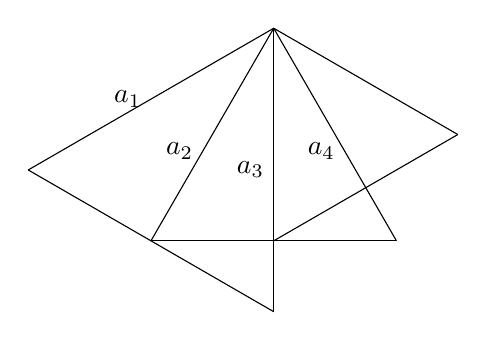
\begin{tikzpicture}[scale=1.8,]
    \foreach \x/\xlen in {-150/2, -120/1.732, -90/2, -60/1.732, -30/1.5}
    {
        \draw(0,0)--(\x:\xlen);
    }
\draw (-150:2)--(-90:2); 
\draw (-120:1.732)--(-60:1.732); 
\draw (-90:1.5)--(-30:1.5); 

\foreach \x in {1,2,3,4}
{
    \node at (-180+30*\x:1)[left]{$a_{\x}$};
}
\end{tikzpicture}
    \caption{}\label{fig:triangle}
\end{figure}


\begin{solution}
  如\cref{fig:triangle},设第 $k$ 个这样的正三角形的边长为 $a_k$,高为 $h_k$, 面积为 $A_k,\; (k=1,2,\ldots,10)$,于是
\[a_1=a,\qquad h_1=\frac{\sqrt{3}}{2}a,\qquad A_1=\frac{1}{2}a_1h_1=\frac{\sqrt{3}}{4}a^2\]
因为所有正三角形都相似,故对应边与对应高线成比例,即
\[\frac{a_{k+1}}{a_{k}}=\frac{h_{k+1}}{h_k}\]
又依三角形的作法,知
\[a_{k+1}=h_k,\qquad (k=1,2,3,\ldots,10)\]
\[\therefore\quad \frac{a_{k+1}}{a_{k}}=\frac{h_{k+1}}{a_{k+1}}=\frac{h_1}{a_1}=\frac{\sqrt{3}}{2}\]
根据相似三角形面积之比等于对应边平方之比,故
\[q=\frac{A_{k+1}}{A_k}=\frac{a^2_{k+1}}{a^2_k}=\left(\frac{a_{k+1}}{a_k}\right)^2=\left(\frac{\sqrt{3}}{2}\right)^2=\frac{3}{4}\]
因此,前 10 个正三角形面积之和
\[S_{10}=\frac{\dfrac{\sqrt{3}}{4}a^2\left[1-\left(\dfrac{3}{4}\right)^{10}\right]}{1-\dfrac{3}{4}}=\sqrt{3}a^2\left[1-\left(\frac{3}{4}\right)^{10}\right]\]
\end{solution}

{\linespread{1.65}\selectfont 为书写简便起见,我们用符号 $\sum\limits^n_{i=m}a_i$ 表示数列 $\{a_i\}$ 的相邻的一些项的和。整数 $i$ 在确定了的界限内变动,在 $\sum$ 的下面和上面的数字分别表示求和的起止项的序号,符号“$\sum$”读作 sigma。例如\par}
\[\begin{split}
    \sum^n_{i=1}a_i&=a_1+a_2+\cdots+a_n\\
    \sum^n_{i=k}a_i&=a_k+a_{k+1}+\cdots+a_n\\
\end{split}\]

在许多数学问题里,我们需要求出以下标 $i$ 的 $k$ 次多项式 $f(i)$ 为通项的前 $n$ 项和的公式:
\[S_k(n)=\sum^{n-1}_{i=0}f(i)=f(0)+f(1)+\cdots+f(n-1)\]
这里的指标集是非负整数集。

数列 $\{S_k(n)\}$ 称为数列 $\{f(n)\}$ 的和数列,即
\[\begin{split}
    S_k(1)&=f(0)\\
    S_k(2)&=f(0)+f(1)\\
    S_k(3)&=f(0)+f(1)+f(2)\\
    \cdots
\end{split}\]

为讨论方便起见,规定 $S_k(0)=0$, 于是和数列 $\{S_k(n)\}$ 满足下面两个性质:
\begin{enumerate}[itemindent=3.5em]
    \item $S_k(0)=0$
    \item $S_k(n+1)-S_k(n)=f(n),\qquad n=0,1,2,\ldots$
\end{enumerate}

我们来考虑这样一个多项式,它在 $k$ 个点 $0,1,2,\ldots,k-1$ 处与横坐标轴相交,又通过 $(k,1)$ 点,显然这个关于 $n$ 的多项式为
\[q_k(n)=\frac{n(n-1)\cdots(n-k+1)}{k!}\]
下面来求数列 $\{q_k(n)\},\; n=0,1,2,\ldots$ 的前 $n$ 项和的公式。

\begin{example}\label{exp:sum_of_qk}
设 $q_k(n)=\dfrac{1}{k!}n(n-1)\cdots(n-k+1)$,则前 $n$ 项的和
\[\begin{split}
    S_k(n)&=\sum^{n-1}_{i=0} q_k(i)=q_k(0)+q_k(1)+\cdots+q_k(n-1)\\
    &=\frac{1}{(k+1)!}n(n-1)\cdots(n-k)
\end{split}\]
换言之,其和是这样一个多项式,它在 $0,1,2,\ldots,(k-1)$,共 $k$ 个点处与坐标轴相交且通过 $((k+1),1)$ 点。
\end{example}

\begin{solution}
设 $S_k(n)$是一个 $n$ 的 $k+1$ 次多项式,且让 $S_k(n)$ 满
足条件:
\begin{align}
    \label{eq:Skn}S_k(0)&=0\\
    \label{eq:Skn+1}S_k(n+1)-S_k(n)&=q_k(n)
\end{align}
由于 $q_k(0)=q_k(1)=\cdots=q_k(k-1)=0$,且 $q_k(k)=1$,于是
\begin{equation}
    \begin{split}
 S_k(n)&=q_k(0)+q_k(1)+\cdots+q_k(n-1)\\
&=\underbrace{0+0+\cdots+0}_{\text{$k$项}}+1+(k+1)+\\
&\qquad \cdots+
\frac{1}{k!}(n-1)(n-2)\cdots(n-k)     
    \end{split}
\end{equation}

由\cref{eq:Skn,eq:Skn+1} 得到
\begin{align}
S_k(0)=S_k(1)=\cdots=S_k(k)=0\\
\label{eq:Skk+1}S_k(k+1)=1
\end{align}
从而知道 $S_k(n)$ 有下面 $k+1$ 个因式,即
\[S_k(n)=Cn(n-1)(n-2)\cdots(n-k)\]
这里 $C$ 是未定的常数因子。

常数因子 $C$ 可由\cref{eq:Skk+1} 确定,
\[S_k(k+1)=C(k+1)k(k-1)\cdots2\cdot 1=1\]
\[\therefore\quad C=\frac{1}{(k+1)!}\]

此处记 $(k+1)!=1\cdot 2\cdot 3\cdots k(k+1)$。

因此,
\[\begin{split}
    S_k(n)&=\sum^{n-1}_{i=0} q_k(i)=\sum^{n-1}_{i=0} \frac{1}{k!}i(i-1)\cdots (i-k+1)\\
    &=\frac{1}{(k+1)!}n(n-1)\cdots (n-k)
\end{split}\]
\end{solution}

我们也常用这样一种想法来求数列前 $n$ 项和的公式,即如果数列的通项能分解成另一个数列相邻两项的差:

$f(n)=F(n+1)-F(n),\; n=0,1,2,\ldots$时,那么前 $n$ 项的和
\[\begin{split}
   S(n)&= \sum^{n-1}_{i=0} f(i)= \sum^{n-1}_{i=0} [F(i+1)-F(i)]\\
   &=[F(1)-F(0)]+[F(2)-F(1)]+\cdots +[F(n)-F(n-1)]\\
   &=F(n)-F(0)
\end{split}\]


\begin{example}
    求 $S(n)=\dfrac{1}{1\cdot 4}+\dfrac{1}{4\cdot 7}+\dfrac{1}{7\cdot 10}+\cdots +\dfrac{1}{(3n-2)(3n+1)}$ 的和。
\end{example}

\begin{solution}
$\because\quad \dfrac{1}{(3i-2)(3i+1)}=\dfrac{1}{3}\left(\dfrac{1}{3i-2}-\dfrac{1}{3i+1}\right)$

\bigskip 当 $i=1,2,3,\ldots,n$ 时,有
\[\begin{split}
    \frac{1}{1\cdot 4}&=\frac{1}{3}\left(\frac{1}{1}-\frac{1}{4}\right)\\
    \frac{1}{4\cdot 7}&=\frac{1}{3}\left(\frac{1}{4}-\frac{1}{7}\right)\\
    \cdots &\cdots\\
    \frac{1}{(3n-2)(3n+1)}&=\frac{1}{3}\left(\frac{1}{3n-2}-\frac{1}{3n+1}\right)
\end{split}\]
因此:
\[\begin{split}
    S(n)&=\sum^n_{i=1}\frac{1}{(3i-2)(3i+1)}\\
    &=\frac{1}{3}\left(\frac{1}{1}-\frac{1}{3n+1}\right)\\
    &=\frac{n}{3n+1}
\end{split}\]
\end{solution}

如果数列的通项是以其它形式的 $k$ 次多项式给出的,我们可以用待定系数法把它变形为\cref{exp:sum_of_qk} 的形式。


\begin{example}
  求 $S_2(n+1)=0^2+1^2+2^2+\cdots+n^2$ 的和。
\end{example}

\begin{solution}
  设 $i^2=\lambda \dfrac{i(i-1)}{2!}+\mu i,\; (i=0,1,2,\ldots,n)$,由待定系数法求得:
\[\lambda=2,\qquad \mu=1\]
于是:
\[S_2(n+1)=\sum^n_{i=0}i^2=2\sum^n_{i=0}\frac{i(i-1)}{2!}+\sum^n_{i=0}i\]
应用\cref{exp:sum_of_qk} 的结果,得到:
\[\begin{split}
    S_2(n+1)&=2\frac{(n+1)n(n-1)}{3!}+\frac{n(n+1)}{2}\\
    &=\frac{n(n+1)(2n+1)}{6}
\end{split}\]
\end{solution}

\begin{example}
设 $a_0,a_1,a_2,\ldots,a_n$ 成等差数列,求 $S_n=a_0+a_1x+a_2x^2+a_3x^3+\cdots+a_nx^n$ 的和。    
\end{example}

\begin{solution}
  \begin{equation}
    \label{eq:sum_anxn}
    S_n=a_0+a_1x+a_2x^2+a_3x^3+\cdots+a_nx^n
  \end{equation}
由于\cref{eq:sum_anxn} 中的系数成等差数列,变量 $1,x,x^2,\ldots,x^n$ 成等比数列,利用等差数列的任意相邻的三项有递归关系:
\begin{equation}
    a_n-2a_{n-1}+a_{n-2}=0,\qquad n\geqslant 2
\end{equation}
知道\cref{eq:sum_anxn} 相邻的三项下面等式成立:
\begin{equation}
  \label{eq:zero_item}
  a_nx^n-2x(a_{n-1}x^{n-1})+x^2(a_{n-2}x^{n-2})=0,\qquad n\geqslant 2
\end{equation}
让\cref{eq:sum_anxn} 的两边分别乘以 $1,-2x,x^2$, 然后相加,得
\[\begin{split}
    S_n&=a_0+a_1x+a_2x^2+a_3x^3+\cdots+a_{n-1}x^{n-1}+a_nx^n\\
    -2xS_n&=-2a_0x-2a_1x^2-2a_2x^3-\cdots-2a_{n-1}x^n-2a_nx^{n+1}\\
    x^2S_n&=a_0x^2+a_1x^3+a_2x^4+\cdots+a_{n-1}x^{n+1}+a_nx^{n+2}
\end{split}\]
所以:
\[(1-x)^2 S_n=a_0+(a_1-2a_0)x+0+\cdots+0+(a_{n-1}-2a_n)x^{n+1}+a_nx^{n+2}\]
由\cref{eq:zero_item} 可知在上面等式中,其余各项为 0,若 $x\neq 1$,两边除以 $(1-x)^2$,得
\[S_n=\frac{a_0+(a_1-2a_0)x+0+\cdots+0+(a_{n-1}-2a_n)x^{n+1}+a_nx^{n+2}}{(1-x)^2}\]
若 $x=1$,原题就变成求等差数列前 $n$ 项的和,这时,
\[S_n=\frac{n(a_1+a_n)}{2}\]
\end{solution}

\begin{example}
    数列 $\{v_n\}$ 由下面递归定义给出:
 \[ v_{n+1}=3v_n-2v_{n-1},\quad v_0=2,\quad v_1=3,\; n=1,2,3,\ldots\]
 求:$v_n$,$S_n=\sum\limits^{n-1}_{i=0}v_i$。
\end{example}

\begin{solution}
    由 $v_{n+1}=3v_n-2v_{n-1}$ 容易看出
  \[  v_{n+1}-v_{n}=2(v_n-v_{n-1})\]
    设 $q_n=v_{n+1}-v_n$,$q_{n-1}=v_n-v_{n-1}$, 则 $q_n=2q_{n-1},\; (n=1,2,\ldots)$,换言之,$\{q_n\}$ 是公比为 2 的等比数列,
\[\therefore\quad q_n=2q_{n-1}=2^2q_{n-2}=\cdots=2^n(v_1-v_0)=2^n(3-2)=2^n\]
从而:
\[\begin{split}
    q_{n-1}&=v_n-v_{n-1}=2^{n-1}\\
v_n&=(v_n-v_{n-1})+(v_{n-1}-v_{n-2})+\cdots+(v_1-v_0)+v_0\\
&=2^{n-1}+2^{n-2}+\cdots +2+1+2\\
&=(2^n-1)+2=2^n+1\\
\end{split}\]
\[\begin{split}
    S_n=\sum^{n-1}_{i=0}v_i&=\sum^{n-1}_{i=0}(2^i+1)=\sum^{n-1}_{i=0}2^i+\sum^{n-1}_{i=0}1\\
    % &=\sum^{n-1}_{i=0}2^i+\sum^{n-1}_{i=0}1\\
    &=(2^n-1)+n=2^n+(n-1)
\end{split}\]
\end{solution}

\begin{Exercise}
\begin{question}
  \item 在等差数列中
  \begin{tasks}(2)
    \task 若 $a_5=100$, $d=\frac{1}{2}$,求$a_{100}$;
    \task 若 $a_3=-4$, $a_5=2$, 求 $a_{10}$;
    \task 若 $a_p=q$, $a_q=p$, 求 $a_{p+q}$;
    \task 用 $a_s$, $a_1$, $d$ 表示 $a_n$。
  \end{tasks}

\item 在 7 和 35 之间插入 6 个数使它们和已给两数组成等差数列。
\item 在 8 和 32 之间应插入多少个等差中项,可使等差中项中的前两个数的和与后两个数的和之比为 $7:25$。
\item 求证含有奇数个项的等差数列里,第一项,中间项,最后项也成等差数列。
\item 在三位数里有几个是 6 的倍数,求它们的和。
\item 求 $S_n=1-2+3-4+5-\cdots+(-1)^{n+1}n$ 的和。
\item 一等差数列前 $n$ 项之和为 $S_n=5n^2+3n$,求 $a_n$。
\item 在等差数列中
\begin{tasks}
  \task 已知 $d=2$, $n=15$, $a_{15}=-10$, 求 $S_{15}$;
  \task 已知 $a_n$, $S_n$ 和 $a_1$,求 $d$;
  \task 已知 $d$, $S_n$ 和 $a_1$,求 $n$;
  \task 已知 $a_n$, $S_n$ 和 $d$, 求 $a_1$。
\end{tasks}

\item 求等差数列 $2\dfrac{1}{2},1\dfrac{5}{6},1\dfrac{1}{6},\ldots$ 的第 $n$ 项,并求这个等差级数的最大和。

\bigskip
\item 在等差数列中,若 $S_1=a_1+a_3+\cdots+a_{2n-1}=44$,$S_2=a_2+a_4+\cdots+a_{2n-2}=33$,求 $a_n$。
\item 某化工厂为了加固烟囱,要在烟囱上打 32 道铁箍,且使每两道铁箍之间的距离相等,已知最上面一道铁箍处烟囱的外直径为 \qty{1.5}{m},最下面一道箍处烟囱的外直径为 \qty{3.5}{m}。求全部铁箍用料的总长。

\item 若 $a_1,a_2,\ldots,a_n$ 成等差数列,求证:
\[\frac{1}{\sqrt{a_1}+\sqrt{a_2}}+\frac{1}{\sqrt{a_2}+\sqrt{a_3}}+\cdots +\frac{1}{\sqrt{a_{n-1}}+\sqrt{a_n}}=\frac{n-1}{\sqrt{a_1}+\sqrt{a_n}}\]

\item 求下列各等比数列的通项公式
\begin{tasks}(2)
    \task $-1,\;-2,\;-4,\;\ldots$
    \task $-1,\;1,\;-1,\;\ldots$
    \task $\dfrac{2}{3},\;\dfrac{1}{2},\;\dfrac{3}{8},\;\ldots$
    \task $\sqrt{2},\;1,\;\dfrac{\sqrt{2}}{2},\;\ldots$
    \task $1,\;-\sqrt{\dfrac{1}{3}},\;\dfrac{1}{3},\;\ldots$
\end{tasks}

\item 在等比数列里
\begin{tasks}
  \task $a_1=36$, $a_5=2\dfrac{1}{4}$,求 $q$ 和 $S_5$;
  \task $a_n=1296$, $q=6$, $S_n=625$,求 $a_0$ 和 $a_1$;
  \task $a_1=3$, $q=\dfrac{1}{3}$, $n=8$,求 $S_8$;
  \task $S_5=242$, $q=3$,求 $a_5$。
\end{tasks}
\item 在等比数列里,若 $a_7-a_5=a_6+a_5=48$, 求 $a_1$, $q$ 和 $S_{10}$。
\item 在 160 和 5 之间插入 4 个数,使这 6 个数成等比数列,求这 4 个数。
\item 求证,若 $a_1,a_2,\ldots,a_n,\ldots\; (a_i>0,i=1,2,3,\ldots)$ 成等比数列,则以下数列均成等比数列:
\begin{tasks}(2)
  \task $a_1,\; a_3,\; \ldots, a_{2n-1},\; \ldots$;
  \task $ka_1,\; ka_3,\; \ldots, ka_{2n-1},\; \ldots$;
  \task $\dfrac{1}{a_1},\; \dfrac{1}{a_2},\; \ldots, \dfrac{1}{a_{n}},\; \ldots$;
  \task $a^2_1,\; a^2_2,\; \ldots, a^2_{n},\; \ldots$;
  \task $\sqrt{a_1},\; \sqrt{a_2},\; \ldots, \sqrt{a_n},\; \ldots$。
\end{tasks}

\item 从盛满 \qty{20}{L} 纯酒精的容器里倒出 \qty{1}{L},然后用水填满,再倒出 \qty{1}{L} 混合溶液,用水填满,这样继续进行,一共倒三次,这时容器里有纯酒精多少?
\item 甲厂产量是乙厂产量的 40.96\%,甲厂产品每年增长的百分率比乙厂产品每年增长的百分率多 30\%,若第四年甲厂产量和乙厂产量相同,求甲厂每年产品平均增长的百分率是多少?
\item 一个机器制造厂的原订的三年计划,每年比上一年增产的机器台数相同,但到了第三年,由于实际需要,须比原计划多生产 1000 台,那么每年比上一年的增长百分数就相同,而且第三年的台数恰为原计划总台数的一半,问实际上每年生产了多少台?每年比上一年增长的百分数是多少?
\item 某农机厂去年十月份生产拖拉机 1000 台,这样连同一月至九月的产量恰好完成全年生产任务,为加速农业机械化,全厂在年底前又生产了 2310 台,于是就超额完成全年计划的 21\%。求
\begin{tasks}
  \task 今年十一、十二月份每月平均增长率;
  \task 今年原计划生产量。
\end{tasks}

\item 若一个三角形的三个角成等差数列,而它的边成等比数列,求这个三角形的形状。
\item 已知一个正三角形边长为 $a$,以此正三角形的高线为边做第二个三角形,依此类推,求前 10 个正三角形的周长的和。
\item 求 $(x+y)+(x^2+xy+y^2)+(x^3+x^2y+xy^2+y^3)+\cdots$ 的前 $n$ 项的和。
\item 求 $7+77+777+\cdots$ 的前 $n$ 项的和。
\item 设等比数列 $a_1,a_2,\ldots,a_n,\ldots$ 的公比是 $q$。求证:$a_1a_2\cdots a_n=a^n_1q^{\tfrac{n(n-1)}{2}}$

\item 求下列各数列的和
\begin{tasks}(3)
    \task $\displaystyle \sum^{n-1}_{i=0} i^3$
    \task $\displaystyle \sum^{n-1}_{i=0} i^4$
    \task $\displaystyle \sum^{n-1}_{i=0} (i-1)i$
    \task $\displaystyle \sum^{n-1}_{i=0} (2i-1)^2$
    \task $\displaystyle \sum^{n-1}_{i=0} \frac{2i+1}{i^2\cdot (i+1)^2}$
\end{tasks}

\item 数列 $a_0,a_1,\ldots, a_n,\ldots$ 中的 $a_0,a_1$ 为已知,且 $a_n=\dfrac{a_{n-1}+a_{n-2}}{2},\; n=2,3,4,\ldots$,求 $a_n$。
\item 数列 $a_1,a_2,\ldots,a_n,\ldots$中,$a_1=2$,且$a_n=3a_{n-1}+1\; (n=2,3,4,\ldots )$, 求 $a_1+a_2+\cdots +a_n$。
\item 已知数列 $a_1,a_2,\ldots ,a_n,\ldots$ 的相邻两项 $a_n$,
$a_{n+1}$ 是方程 $x^2+3nx+c_n=0,\; (n=1,2,\ldots)$ 的两根,当 $a_1=1$ 时,求 $\sum\limits^{2p}_{n=1}c_n$。
\item $n$ 是非负的整数,试问同时满足下面三个不等式的整数对 $(x,y)$ 共有多少组?
\[y\geqslant x,\qquad y\leqslant 3x,\qquad y\leqslant n\]
\item 三角形三条边的长分别是$\ell$, $m$ 和 $n$,这里 $\ell$,$m$,
$n$都是正整数,且$\ell\leqslant m\leqslant n$,对于每一个给定的$n$(取
$n=1,2,3,\ldots$),所说的不同形状的三角形有多少个?求
出三角形的个数用 $n$ 表示的一般公式。
\item 数列 $\{a_n\}$ 是:
\[a_1=\frac{1}{3},\qquad \frac{1}{a_{n+1}}-\frac{1}{a_n}=2n+3\quad (n=1,2,3,4,\ldots)\]
\begin{tasks}
  \task 用 3 的式子表示一般项;
  \task 用 $n$ 的式子表示前 $n$ 项的和 $\displaystyle\sum^n_{k=1}a_k$
\end{tasks}

\item 若数列 $\{a_n\}$ 是等差数列,
求证:\[\frac{1}{a_1a_2}+\frac{1}{a_2a_3}+\cdots+\frac{1}{a_{n-1}a_n}=\frac{n-1}{a_1a_n}\]
\end{question}
\end{Exercise}

\section{数学归纳法}
现在我们研究在数学中常用的一种证明方法——数学归纳法。

我们常常从一些特殊事实归纳出一般结论,这种推理方法就是通常说的归纳法,用归纳法可以帮助我们从特殊情况发现一般规律,但如果归纳时所根据的特殊事实没有完全包括结论中所涉及到的所有情况,结论可能不正确,这就是说:命题可能对于一系列的特别情形是对的,但是一般并不正确。

例如,已知函数 $f(n)=(n^2-5n+5)^2$,则
\[f(1)=1,\qquad f(2)=1,\qquad f(3)=1,\qquad f(4)=1 \]
如果我们由此得出结论 $f(n)=(n^2-5n+5)^2=1$ ($n$ 是任何自然数),那就是错误的,事实上,$f(5)=25$,不等于1。

为了克服这种归纳法的不完全性,我们常采用下述的数学归纳法来证明一个关于自然数 $n$ 的命题。

数学归纳法的证明逻辑是:

对于一个依赖于自然数 $n=1,2,3,\ldots$ 的命题 $p(n)$,如果
\begin{enumerate}
  \item 当 $n=1$ 时,命题 $p(1)$ 正确;
  \item 假设 $n=k,\; (k\geqslant 1)$ 时,命题 $p(k)$ 正确,可以推出 $n=k+1$ 时,命题 $p(k+1)$ 正确,那么,命题 $p(n)$ 对于一切自然数 $n=1,2,3,\ldots$ 都正确。
\end{enumerate}

这个方法的根据,就是自然数的基本性质:

\begin{Theorem}[自然数的基本性质]{性质}
  令 $A$ 是自然数集 $\mathbb{N}$ 中具有下面性质的子集:
\begin{enumerate}
  \item\label{itm:prop1} $1\in A$;
  \item\label{itm:prop2} 若 $n\in A$,则 $n+1\in A$
\end{enumerate}
那么:$A=\mathbb{N}$。
\end{Theorem}

现在,我们来证明数学归纳法的正确性,设使命题 $p(n)$ 成立的自然数是自然数集 $\mathbb{N}$ 中的子集 $A$,即 $A\subseteq \mathbb{N}$。

根据数学归纳法中的 \ref{itm:prop1},$1\in A$; 再根据数学归纳法中的 \ref{itm:prop2},若 $n\in A$,则 $n+1\in A$。于是,根据自然数的基本性质,得到
\[A=\mathbb{N}\]
因此,命题 $p(n)$ 对于一切自然数成立。

下面举一些例子说明这个方法的应用。

\begin{example}
  求证:
  \begin{equation}
    \label{eq:sum_n}
    1+2+3+\cdots+n=\frac{n(n+1)}{2}
  \end{equation}
\end{example}

\begin{analyze}
    我们注意到和式:$1+2+3+\cdots+n$ 可以递归地定义为
\[\begin{cases}
    S(1)=1\\
    S(n)=S(n-1)+n,\qquad n=2,3,\ldots
\end{cases}\]
上面的等式为应用数学归纳法去证明打下了基础。
\end{analyze}

\begin{proof}
  \begin{enumerate}
    \item\label{itm:proof1} 当 $n=1$ 时,$\because\, S(1)=1,\quad \dfrac{1\times(1+1)}{2}=1$,$\therefore\, $ \cref{eq:sum_n} 成立。
    \item\label{itm:proof2} 假设 $n=k,\; (k\geqslant 1)$ 时,\cref{eq:sum_n} 成立,即有
\[S(k)=1+2+3+\cdots+k=\frac{k(k+1)}{2}\]
那么,当 $n=k+1$ 时,
\[S(k+1)=1+2+3+\cdots+k+(k+1)=S(k)+(k+1)\]
应用数学归纳法假设于上面的等式,得到
\[\begin{split}
    S(k+1)&=\frac{k(k+1)}{2}+(k+1)=(k+1)\left(\frac{k}{2}+1\right)\\
    &=\frac{(k+1)(k+2)}{2}\\
    &=\frac{(k+1)[(k+1)+1]}{2}
\end{split}\]
即\cref{eq:sum_n} 仍成立。

由所证 \ref{itm:proof1} 和 \ref{itm:proof2} 两步知:
\[1+2+3+\cdots+n=\frac{n(n+1)}{2}\]
对于一切自然数 $n$ 都成立。
\end{enumerate}
\end{proof}

从上例明显地看出,用数学归纳法证明一个命题的步骤是:
\begin{enumerate}
\item\label{itm:stp1} 验证命题 $p(n)$,当 $n$ 取第一个值 $n=1$ 时,$p(1)$ 正
确。这一条是数学归纳法的基础。
\item\label{itm:stp2} 假设当 $n=k,\; (k\geqslant 1)$时,命题 $p(k)$ 正确,证明当 $n=k+1$ 时,命题 $p(k+1)$ 也正确。这一条是说性质 $p(n)$ 具有遗传性,可以一代一代地传下去。完成了这两步以后,就可以断定命题 $p(n)$ 对于一切自然数 $n$ 都正确。因为首先证明 $p(1)$ 正确,另外由 $p(1)$ 正确推出 $p(2)$ 正确,由 $p(2)$ 正确推出了 $p(3)$ 正确,依次下去,便可知对于一切自然数 $n$,$p(n)$ 正确。
\end{enumerate}


有时不一定从 1 开始,也就是数学归纳法里两句话,可以改成
\begin{enumerate}
  \item 当 $n=k_0$ 时,命题 $p(k_0)$ 正确。
  \item 从假设 $n=k,\; (k\geqslant k_0)$ 时,这个命题 $p(k)$ 正确,可以推出当 $n=k+1$ 时,这个命题 $p(k+1)$ 也正确,那么 $p(n)$ 对于 $n\geqslant k_0$ 都正确。
\end{enumerate}

\begin{example}
  假设我们只有面额是 3 分和 5 分的两种邮票,试证明可以用面额是 3 分和 5 分的两种邮票去付多于 7 分的任意一
笔邮资。

如果我们对于每一种情形逐一地去证明,譬如,用 3 分和 5 分的邮票各一张可以付 8 分的邮资;用 3 分的邮票 3 张可以付 9 分的邮资,用 5 分的邮票 2 张可以付 10 分的邮资等等,照这样一个一个地验证下去,不是有成效的,因为有无数多种的情况需要去验证,让我们用数学归纳法来证明。
\end{example}

\begin{proof}
\begin{enumerate}
  \item\label{itm:exstep1} 我们对于 8 分的邮资,可以用 3 分和 5 分的邮票各一张去付,因此,当 $n=8$ 时,命题正确。
  \item\label{itm:exstep2} 假设用 3 分邮票和 5 分的邮票可以付 $k$ 分的邮资,我们要证明这两种邮票也可以用来付 $k+1$ 分的邮资。

  因为 $k\geqslant 8$,有两种可能的情形:$k$ 分的邮资至少要用一张 5 分的邮票去付;$k$ 分的邮资完全可以用 3 分的邮票去付。

  在第一种情形下,要付 $k+1$ 分的邮资,只要原来的某一张 5 分的邮票换以两张 3 分的邮票就可以了;

  在第二种情形下,3 分的邮票至少要有 3 张。要付 $k+1$ 分的邮资,只要把原来的三张 3 分邮票换以两张 5 分的邮票就可以了。

  根据 \ref{itm:exstep1} 和 \ref{itm:exstep2},可以断定 $n$ 为任何大于 7 的自然数,命题正确。
\end{enumerate}

\bigskip
数学归纳法这两步骤,是缺一不可的,从求函数 $f(n)=(n^2-5n+5)^2$ 的值可知,缺少了步骤 \ref{itm:stp2} 就得出不正确的结论,同样缺少了步骤1也可能得出不正确的结论。例如,由于没有验证数学归纳法中的第一条,而得出下面荒谬的结论:
\[2+4+6+\cdots+2n=n^2+n+1\]

我们在下面只证明数学归纳法中的 \ref{itm:stp2}。

假设 $n=k,\; (k>1)$,等式 $2+4+6+\cdots+2k=k^2+k+1$ 成立,那么,当 $n=k+1$ 时,
\begin{align*}
    2+4+6+\cdots+2k+2(k+1)&=(2+4+6+\cdots+2k)+2(k+1)\\
&=k^2+k+1+2(k+1)  \tag{数学归纳法假设}\\
&=(k+1)^2+(k+1)+1
\end{align*}
由此知,当 $n=k+1$ 时,等式仍成立。如果仅从数学归纳法中的 \ref{itm:stp2} 就得出等式对于任何自然数都成立,那是错误的。

事实上,当 $n=1$ 时,等式左边 $=2$,右边 $=1^2+1+1=3$,因此,上面的等式是错误的。
\end{proof}

\begin{example}
    证明:
\[S(n)=1-2^2+3^2-4^2+\cdots+(-1)^{n-1}n^2=(-1)^{n-1}\frac{n(n+1)}{2}\]
\end{example}

\begin{proof}
\begin{enumerate}
    \item 当$n=1$时,$S(1)=1$,又$(-1)^0\frac{1(1+1)}{2}=1$,所以等式成立。

\item 假设$n=k$时,有
\[S(k)=1-2^2+3^2-4^2+\cdots+(-1)^{k-1}k^2=(-1)^{k-1}\frac{k(k+1)}{2}\]
那么,当$n=k+1$时,有    
\[\begin{split}
    S(k+1)=S(k)+(-1)^k(k+1)^2&=(-1)^{k-1}\frac{k(k+1)}{2}+(-1)^k(k+1)^2\\
    &=(-1)^k(k+1)\left[-\frac{k}{2}+(k+1)\right]\\
    &=(-1)^k \frac{(k+1)(k+2)}{2}\\
    &=(-1)^k \frac{(k+1)[(k+1)+1]}{2}
\end{split}\]
\end{enumerate}

由1和2知,等式对于一切自然数 $n$ 都成立。
\end{proof}


\begin{example}
证明:
\[\begin{split}
    S(n)&= \sin \alpha+\sin (\alpha+\beta)+\sin (\alpha+2 \beta)+\cdots+\sin (a+(n-1) \beta) \\
&= \dfrac{\sin(n\beta/2)}{\sin(\beta/2)} \sin \left(\alpha+\dfrac{n-1}{2} \beta\right)
\end{split}\]
\end{example}

\begin{proof}
\begin{enumerate}
    \item\label{itm:proof1_triangle} 当 $n=1$ 时,
\[\because\, \text{左边}=S(1)=\sin\alpha,\quad \text{右边}=\dfrac{\sin(\beta/2)}{\sin(\beta/2)}\sin(\alpha+0\cdot \beta)=\sin\alpha, \quad\therefore\, \text{等式成立。}\]
% $\therefore\quad $ 等式成立。

\item\label{itm:proof2_triangle} 假设 $n=k$ 时,
\[\begin{split}
    S(k)&=\sin \alpha+\sin (\alpha+\beta)+\sin (\alpha+2 \beta)+\cdots+\sin (\alpha+(k-1) \beta) \\
&=\dfrac{\sin(k\beta/2)}{\sin(\beta/2)} \sin \left(a+\dfrac{k-1}{2} \beta\right)
\end{split}\]
成立,那么:
\[\begin{split}
    S(k+1)&= S(k)+\sin(\alpha+k\beta)\\
    &=\dfrac{\sin(k \beta/2)}{\sin(\beta/2)} \sin \left(a+\dfrac{k-1}{2} \beta\right)+\sin(\alpha+k\beta)\\
    &=\frac{1}{\sin(\beta/2)}\left[\sin\left(\alpha+\frac{k-1}{2}\beta\right)\sin\frac{k\beta}{2}+\sin(\alpha+k\beta)\sin\frac{\beta}{2}\right]\\
    &=\frac{1}{2\sin(\beta/2)}\left[\cos\left(\alpha-\frac{\beta}{2}\right)-\cos\left(\alpha+k\beta-\frac{\beta}{2}\right)\right. \\
    &\qquad \qquad \left. +\cos\left(\alpha+k\beta -\frac{\beta}{2}\right)-\cos\left(\alpha+k\beta+\frac{\beta}{2}\right)\right]\\
    &=\frac{1}{2\sin(\beta/2)}\left[\cos\left(\alpha-\frac{\beta}{2}\right)-\cos\left(\alpha+k\beta+\frac{\beta}{2}\right)\right]\\
    &= \frac{(-2)}{2\sin(\beta/2)}\sin\left(\frac{2\alpha+k\beta}{2}\right)\sin\left(\frac{-k\beta-\beta}{2}\right)\\
    &=\frac{1}{\sin(\beta/2)}\cdot \sin\left(\alpha+\frac{k}{2}\beta\right)\cdot \sin\frac{(k+1)\beta}{2}\\
    &=\frac{\sin[(k+1)\beta/2]}{\sin(\beta/2)}\sin\left[\alpha+\frac{(k+1)-1}{2}\beta\right]
\end{split}\]
即当 $n=k+1$ 时,等式仍成立。由 \ref{itm:proof1_triangle} 和 \ref{itm:proof2_triangle} 可知,等式对任何自然数 $n$ 都成立。
\end{enumerate}
\end{proof}

\begin{example}
  用数学归纳法证明,如果 $n$ 是一个正整数,那么 $x^{2n}-y^{2n}$ 能被 $x+y$ 整除。
\end{example}

\begin{proof}
\begin{enumerate}
    \item\label{itm:proof1_devision} 当 $n=1$ 时,$x^2-y^2=(x+y)(x-y)$ 能被
    $x+y$整除。
    \item\label{itm:proof2_devision} 假设当 $n=k$,($k$ 是自然数),$x^{2k}-y^{2k}$ 能被 $x+y$ 整除,那么当 $n=k+1$ 时,
\[\begin{split}
    x^{2(k+1)}-y^{2(k+1)}
    &=x^2\cdot x^{2k}-y^2\cdot y^{2k}\\
    &=x^2\cdot x^{2k}-x^2y^{2k}+x^2y^{2k}-y^2\cdot y^{2k}\\
    &=x^2(x^{2k}-y^{2k})+(x^2-y^2)\cdot y^{2k}
\end{split}\]
    
    因为 $x^{2k}-y^{2k}$ 与 $x^2-y^2$ 都能被 $x+y$ 整除,所以 $x^2(x^{2k}-y^{2k})+(x^2-y^2)y^{2k}$ 也能被 $x+y$ 整除,这就是说,$x^{2k+1}-y^{2k+1} $能
    被$x+y$整除。
\end{enumerate}  

根据 \ref{itm:proof1_devision} 和 \ref{itm:proof2_devision},命题成立。
\end{proof}

\begin{example}\label{exp:lines}
    平面上有 $n$ 条直线,其中任何两条不平行,任何
三条不过同一点,证明这 $n$ 条直线把平面分成 $f(n)=\dfrac{1}{2}
(n^2+n+2)$ 个部分。
\end{example}

\begin{proof}
\begin{enumerate}
    \item\label{itm:proof1_lines} 当 $n=1$ 时,直线把平面分成两部分(为了简单起见,也说分成两块),又
  \[f(1)=\frac{1}{2}(1^2+1+2)=2\]
    因此,$n=1$ 时命题成立。
   \item\label{itm:proof2_lines} 假设 $n=k$ 时命题成立,就是
\[f(k)=\frac{1}{2}(k^2+k+2)\]

我们要设法找出 $f(k+1)$ 与 $f(k)$ 的递归关系,即由$f(k)$ 求得 $f(k+1)$ 的关系。为此,我们在平面上再增加一条直线 $\ell$(\cref{fig:lines}),
\begin{figure}
  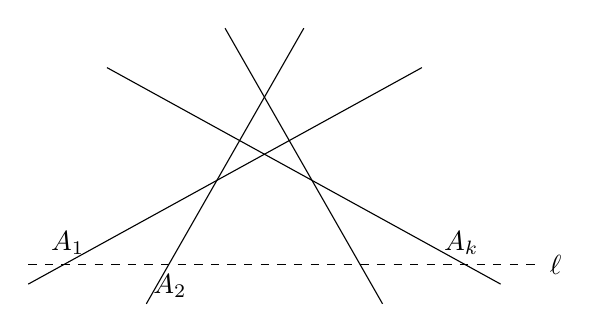
\begin{tikzpicture}%[very thick]
    \draw (1.5,-1)--(-.5,2.5);
    \draw (-1.5,-1)--(.5,2.5);
    \draw (-3,-.75)--(2,2);
    \draw (3,-.75)--(-2,2);
    \node at (-2.5,-.5) [above] {$A_1$};
    \node at (-1.2,-.5) [below] {$A_2$};
    \node at (2.5,-.5) [above] {$A_k$};
    \draw[dashed] (-3,-.5)--(3.5,-.5)node[right]{$\ell $};
  \end{tikzpicture}
  \caption{}\label{fig:lines}
\end{figure}
因为已知任何两条直线不平行,所以直线 $\ell$ 与平面上的原 $k$ 条直线都相交,而且这 $k$ 个交点互不相同,否则与任何三条直线不过同一点的已知条件矛盾,这 $k$ 个交点将直线 $\ell$ 分成 $k+1$ 段,因此直线 $\ell$ 越过原来的 $k+1$ 块平面部分,直线上的每段将它所在的原平面块分成两块,因此要给原来的平面部分的总数 $f(k)$ 增加 $k+1$ 块新的平面部分,就是
\[f(k+1)=f(k)+(k+1)\]
将 $f(k)=\dfrac{1}{2}(k^2+k+2)$ 代入上式,得到
\[\begin{split}
    f(k+1)&=\frac{1}{2}(k^2+k+2)+(k+1)\\
    &=\frac{1}{2}(k^2+3k+4)\\
    &=\frac{1}{2}[(k+1)^2+(k+1)+2]
\end{split}\]
这就是说,当 $n=k+1$ 时,命题也成立。



根据 \ref{itm:proof1_lines} 和 \ref{itm:proof2_lines},可知命题成立。
\end{enumerate}
\end{proof}

同学也许会问:\cref{exp:lines} 的结果是怎样发现的?数学归纳法能解决这个问题吗?其实此题的证明已经解决了这个问题,因为我们证明了 $f(n)$ 可以递归地定义为
\[\begin{cases}
    f(1)=2\\
    f(k+1)=f(k)+(k+1),\qquad k=1,2,\ldots,(n-1)
\end{cases}\]

首先 $f(1)$ 有定义,其次如果知道了 $f(1)$,就知道 $f(2)$,依次推下去,就知道$f(n)$。所以
\[\begin{split}
  f(n)&=[f(n)-f(n-1)]+[f(n-1)-f(n-2)]+\cdots +[f(2)-f(1)]+f(1)\\
  &=n+(n-1)+\cdots +2+2\\
  &=[n+(n-1)+(n-2)+\cdots +2+1]+1\\
  &=\frac{n(n+1)}{2}+1=\frac{n^2+n+2}{2}  
\end{split}\]


\begin{Exercise}
\begin{question}
    \item 用数学归纳法证明下列各等式: 
\begin{tasks}(2)
    \task $\displaystyle\sum^n_{k=1}3^{k-1}=\frac{3^n-1}{2}$
    \task $\displaystyle\sum^n_{k=1}k(k+1)=\frac{1}{3}n(n+1)(n+2)$
    \task $\displaystyle\sum^n_{k=1}\frac{1}{k(k+1)}=\frac{n}{n+1}$
    \task! \[\sum_{i=1}^{n}\cos[\alpha+(i-1)\beta]=\frac{\sin\dfrac{n\beta}{2}}{\sin\dfrac{\beta}{2}}\cos\left(\alpha+\frac{n-1}{2}\beta\right)\]
\end{tasks}

\item 用数学归纳法证明:
\begin{tasks}
\task 当 $n$ 是正整数时,$x^n-y^n$ 能被 $x-y$ 整除。
\task 当 $n$ 是正奇数时,$x^n+y^n$ 能被 $x+y$ 整除。
\task $(3n+1)7^n-1$ 能被 9 整除。
\task 邻近的三个自然数的立方和,必定能被 9 整除。
\task 当 $n$ 是正整数时,$(11)^{n+2}+(12)^{2n+1}$ 能被 133 整除。
\task 当 $n$ 是正整数时,$3^{2n+2}-8n-9$ 能被 64 整除。
\end{tasks}

\item 数列 $\{a_n\}$ 是这样确定的:
\[a1=1,\quad 4a_ka_{k+1}=(a_k+a_{k+1}-1)^2,\quad a_k<a_{k+1}\quad (k=1,2,3,\ldots)\]
\begin{tasks}
  \task\label{tsk:equation} 求 $a_2,a_3,a_4$, 并由此推断 $a_n$;
  \task 用数学归纳法证明 \ref{tsk:equation} 中推断出的 $a_n$ 的正确性。
\end{tasks}

\item 空间有$n$个平面,其中没有两个平面平行,没有三个平面相交于同一条直线,也没有四个平面过同一个点。求证:它们把空间分成 $f(n)=\frac{1}{6}(n^3+5n+6)$ 份。
\item 有 $n$ 个圆,其中每两个圆都相交于两点,并且每三个圆不相交于同一点。求证:这 $n$ 个圆把平面分成 $n^2-n+2$ 部分。
\item 若数列 $\{a_n\}$,当 $n\geqslant 3$ 时,满足条件
\[\frac{1}{a_1a_2}+\frac{1}{a_2a_3}+\frac{1}{a_3a_4}+\cdots+\frac{1}{a_{n-1}a_n}=\frac{n-1}{a_1a_n}\]
用数学归纳法证明数列 $\{a_n\}$ 是等差数列。
\end{question}
\end{Exercise}